\chapter{Umsetzung}
\label{chap:umsetzung}
    Im Rahmen einer prototypischen Implementierung wurde das im Konzept (siehe Kapitel \ref{chap:konzept}) geplante System
    umgesetzt. Gegenstand dieses Kapitels wird es sein, Aspekte der Umsetzung widerzuspiegeln und konkret die Umsetzung eines  
    Anwendungsfalls darzulegen. Zusätzlich wird die Auswahl des dafür genutzten Frameworks aufgegriffen. 

\section{Auswahl des Frameworks}
\label{sec:frameworkauswahl}
    Im Bereich der Java-Entwicklung gibt es mittlerweile viele Möglichkeiten, um Applikationen, Anwendungen und Frameworks 
    zu entwickeln, die unterschiedliche Präferenzen und Einsatzmöglichkeiten bieten. Dadurch sind, auf den Einsatzbereich bezogen, 
    Vor- und Nachteile im Vergleich ähnlicher Systeme nicht auszuschließen. Eine kleine Auswahl an Systemen wurde getestet und auf deren 
    Brauchbarkeit analysiert und evaluiert. Für diese Evaluation wurden Kriterien ausgearbeitet, mit der die Auswahl des Frameworks 
    eingeschränkt und nach Möglichkeit das passende ergeben soll. Die Kriterien sind nach ihrer Relevanz aufgelistet: 
    \begin{enumerate}
        \item Freiheiten bei der Nutzung (Anwendung und Gewährleistung von Entwurfsmustern).
        \item Nutzung und Bereitstellung von Bibliotheken (Libraries).
        \item Bereitstellung einer Plattform (Full Stack).
        \item Aktive Community und stetige Weiterentwicklung des Systems.
        \item Nutzung des Frameworks in bereits bestehenden Projekten im Bereich Smart Home.
        \item Open Source-Projekt, um Flexibilität und weitestgehende Unabhängigkeit zu gewährleisten.
        \item Ausschluss von Frameworks, die ausschließlich für die Web-Entwicklung gedacht sind.
    \end{enumerate}  
    Aufgrund der Vielzahl an Frameworks war es im Rahmen dieser Arbeit nicht möglich, alle vorhandenen und in Betracht 
    gezogenen Systeme detailliert aufzuführen. Lediglich die engere Auswahl wird aufgegriffen. 
    Nach ausführlicher Recherche und unter Berücksichtigung von Frameworks, wie bspw. Grails, Quarkus, Blade, und Play, wurden 
    schließlich genau zwei Systeme genauer betrachtet, die die vorangestellten Kriterien in Gänze erfüllen. Viele in Erwägung gezogene Frameworks 
    finden überwiegend in der Web-Entwicklung Anwendung, bzw. basieren auf dem Spring Framework. Durch diese Erkenntnis wurden 
    viele Systeme nicht weiter berücksichtigt. Die beiden Kernsysteme, die ihren Einsatz und ihre Möglichkeiten rechtfertigen
    werden in den folgenden Abschnitten kurz erläutert.

    \subsection{OSGi}
    \label{subsec:osgiFramework}
        Das \ac{OSGI} Framework der \acs{OSGI}\footnote{Ursprung der OSGi Plattform. \url{https://www.osgi.org/about/} Abgerufen am 19.06.2022} 
        Alliance, welches in der openHAB Software eingesetzt wird, klassifiziert eine dynamische Softwareplattform, mit der die Modularisierung 
        und Verwaltung von Applikationen und den dazugehörigen Diensten mittels Komponentenmodell realisiert werden kann \cite{funke2009}. Bekannte 
        Produkte, die auf der \acs{OSGI} Plattform laufen, sind neben openHAB unter anderem die Entwicklungsumgebung Eclipse der Eclipse 
        Foundation, Produkte und Softwarelösungen von IBM, Oracle, Adobe und weitere. 
        \\
        Nennenswerte Eigenschaften und Vorteile der Software sind die Modularisierung und Versionierung, das zur Laufzeit organisierte 
        Abhängigkeitsmanagement, das Fernmanagement des laufenden Systems über sogenannte Management Agents und die Nutzung des 
        Serviceorientierten Programmiermodells, \ac{SOA}\footnote{Erläuterung des SOA Modells. \url{https://www.ibm.com/cloud/learn/soa} Abgerufen am 20.06.2022}. 
        An dieser Stelle wird das Framework nicht technisch vertieft. Die Funktionsweise und die technisch 
        fundierte Erläuterung kann dem Buch \cite{osgibuch}, sowie der Dokumentation \cite{osgipraesentation} eines ausgearbeiteten Workshops entnommen werden. 
        Nachteile der Plattform sind zum einen der weniger breite Einsatz des Frameworks und zum anderen die kleine Community. 
        Ebenso findet eine Weiterentwicklung der Plattform nur mäßig statt. Dies hat zur Folge, dass die Erweiterung, bzw. die Entwicklung des darauf 
        aufbauenden Systems träge vonstattengeht. 
        %Wieso Spring Boot und nicht OSGi?
        %Wieso Java und nicht Python oder andere?

    \subsection{Spring}
    \label{subsec:springBootFramework}
        Spring\footnote{Open-Source-Framework Spring. \url{https://spring.io} Abgerufen am 02.07.2022} ist ein Open-Source-Framework, welches auf der Java-Plattform aufbaut. 
        Das Ziel von Spring selbst ist die Vereinfachung und Förderung von Programmierpraktiken in der Java- und Java EE Entwicklung. Mit einem breiten Spektrum an 
        Funktionalitäten bietet das Framework eine ganzheitliche Lösung zur Entwicklung von Applikationen, Anwendungen und Frameworks. Im Vordergrund dabei steht immer die 
        Entkopplung von Applikationskomponenten. Das Spring Framework wurde im März 2004 offiziell Freigegeben und wird seitdem stetig weiterentwickelt. 
        Initiator des Frameworks ist der Author und Softwareentwickler Rod Johnson. Das Framework, welches in dem Buch des Experten Rod Johnson erläutert wird, basiert auf 
        den folgenden Prinzipien \cite{johnson2004expert}: 
        \\
        \linebreak
        Dependency Injection ist ein sehr bekanntes Entwurfsmuster. Dabei werden die Abhängigkeiten eines Objektes zur Laufzeit reglementiert. Unter 
        Verwendung des Frameworks werden den Objekten die benötigten Objekte und Ressourcen zugewiesen. Dadurch müssen diese nicht selbst gesucht werden. 
        \\
        \linebreak
        Ein weiterer Punkt ist die aspektorientierte Programmierung, durch die der Entwickler technische Aspekte voneinander isolieren und den eigentlichen Programmcode 
        von Transaktionen oder anderen Faktoren freizuhalten. 
        \\
        \linebreak
        Das dritte Prinzip ist das Bereitstellen von Vorlagen zur Vereinfachung der Nutzung von Schnittstellen, sog. \acs{API}s. Dadurch wird ein POJO-basiertes Modell 
        möglich. Unter POJO, \textit{Plain Old Java Object}, ist ein ganz normales Objekt in Java zu verstehen. 
        \\
        \linebreak
        Zusammenfassend sind beide Frameworks dazu geeignet, um das Konzept der Steuerzentrale unterstützend zu realisieren. 
        Ein direkter Vergleich zwischen den Frameworks kann nicht gezogen werden, da die Funktionalitäten, bzw. die aus der Nutzung 
        profitablen Eigenschaften nicht vergleichbar sind. Während sich Spring auf die Unterstützung zur Erstellung von Applikationen konzentriert, 
        legt \acs{OSGI} den Mehrwert auf die Modularisierung durch Kontainerisierung. Durchaus ist eine Kombination aus beiden 
        Frameworks möglich, um Vorteile beider zu vereinen. Fundamental bietet Spring jedoch weitaus mehr Möglichkeiten und Unterstützungen 
        zur Entwicklung von Applikationen und Frameworks, weshalb es im Rahmen dieser Arbeit eingesetzt wird. Mit Spring Boot, welches auf Spring 
        aufbaut können auch \acl{MVC} Web-Architekturen und \acs{REST} \acs{API}s implementiert werden. So kann mit dieser Entscheidung 
        ein Vollumfängliches System erstellt werden. Unter zusätzlicher Verwendung von \acs{OSGI} wäre eine weiter Modularisierung und Kontainerisierung möglich. Dies 
        ist auch durch Spring mit Hilfe von Microservices in einer anderen Form realisierbar. 
        \\
        An der Stelle wird im Rahmen dieser Arbeit das Thema von Microservices und Kontainerisierung nicht weiter konkretisiert.
        \\
        \linebreak
        Die Entscheidung viel auf Spring, da dieses ein modernes und etabliertes Framework darstellt und die 
        Community erheblich größer ist, als die des \acs{OSGI} Frameworks. Hinzukommt, die Schaffung eines alternativen Ansatzes zu openHAB, da dieses System bereits 
        auf \acs{OSGI} aufbaut. 
        Dennoch unterscheidet sich die Steuerzentrale in den Funktionalitäten und Angeboten immens im Vergleich zu openHAB. Das System bietet weitaus mehr 
        Funktionalitäten, Erweiterungen und Ausprägungen. Lediglich kann zum Vergleich die Definition von Regeln herangezogen werden. 

\section{Implementierung}
\label{sec:implementation}
    Hierbei wird konkret die Implementierung des Frameworks aufgegriffen und beschrieben, wie Konzeptentscheidungen im Code umgesetzt wurden. 
    Auch werden wichtige Anhaltspunkte ergänzt, die in der Tiefe nicht aus dem Konzept hervorgehen, da sich dort lediglich auf die Idee und die allgemein gehaltene 
    Vorstellung bezogen wurde. 

\subsection{Generische Programmierung} % Typisierung
\label{subsec:java_generics}
% Erledigt! -> WICHTIG!!!: Verwendung der Typisierung, um dem Anwender die Möglichkeit der offenen Gestaltung des Zustandobjektes zu gewährleisten.
    Eine entscheidende Überlegung der Umsetzung in Richtung des Zustandsraumes ist die Verwendung der generischen Programmierung. 
    Mit dem Hintergrund, dass der Entwickler die volle Entscheidungsmacht über die Implementierung der 
    Regeln, des Zustandsraumes und den dafür notwendigen Bedingungen beibehält, ist die Überlegung  
    notwendig, wie mit einem Objekt gearbeitet werden kann, ohne dass es vor der Systemlaufzeit bekannt ist. 
    \\
    \linebreak
    Hierfür wird auf das Konzept der generischen Programmierung, sog. \textit{Generics}, gesetzt. Ein Synonym 
    des Begriffs ist der \textit{parametrisierte Typ}. Mit der Nutzung von Generics ist ein syntaktisches Mittel 
    gegeben, mit dem Klassen und Methoden mit Typen parametrisiert werden können. Diese Typ-Variablen sind zum 
    Zeitpunkt der Implementierung unbekannt und können beliebig definiert werden. Erst zur Laufzeit des Systems 
    wird die Typ-Variable durch ein Objekt ersetzt. Somit ist zur Laufzeit das 
    Objekt, dessen Struktur, Methoden und Funktionen bekannt. Bei der Verwendung von generischen Typen gibt es 
    Varianzfälle, die unterschiedliche Auswirkungen aufzeigen. Der für das Konzept relevante Fall ist der des 
    einfachen Typ-Parameters. Weitere Varianzfälle werden in dieser Ausarbeitung nicht erläutert. 
    \\
    \linebreak
    Ein konkretes Anwendungsbeispiel, wie es 
    auch im Rahmen dieser Arbeit verwendet wird, sieht wie folgt aus:
    \\
    Das Framework arbeitet mit dem generischen Typ \textit{E}. Der Anwender soll nach der Implementierung der Klasse des Zustandsraumes das 
    jeweilige Objekt dem Framework übergeben. So ist zur Laufzeit das konkrete Objekt bekannt. Zur Veranschaulichung dient folgendes Code-Beispiel:
\begin{lstlisting}[language=Java, frame=lines, xleftmargin=\parindent, style=algoBericht, label={code:generics}, captionpos=b, caption={Zustandsobjekt als Typ-Variable}]
public class LogicHub<E> {
    private E state;
    ...
    public E getState() {
        return this.state();
    }
}

public class Application {
    private final LogicHub<InnovationLab> logicHub;

    public static void main(String[] args) {
        logicHub = LogicHub.getInstance();
        logicHub.getState(); // -> returns the state object 
                             // and it's values.
    }
}
\end{lstlisting}
    Mit den Java Generics ist eine leistungsstarke Ergänzung der Java-Sprache gegeben, da es die Arbeit des Programmierers einfacher und 
    weniger Fehleranfällig macht. Zusätzlich wird durch die Generics die Typkorrektheit zur Kompilierzeit erzwungen und ermöglicht 
    die Implementierung generischer Algorithmen, ohne für Anwendungen einen zusätzlichen Overhead zu verursachen. 
    \\
    Mit der Option des generischen Typs kann das Framework universell definiert und der Zustandsraum vom Anwender individuell implementiert werden.
    \\
    \linebreak
    Durch die Verwendung der Java Generics wird der konzeptionelle Schnitt zwischen Framework und Anwender-Interaktionen im Quellcode deutlicher.
%Die Darstellung des Zustandsobjektes wird als bereits bestehendes vorausgesetzt, um die folgenden Diagramme vollständig und sinngemäß wiederzugeben. 
%Diese beschreiben jedoch zu keinem Zeitpunkt eine konkrete Struktur des Zustandsobjektes. 
%\\
%\linebreak
%Im weiteren Verlauf wird der Aufbau des Frameworks erläutert, sowie die detaillierte Beschreibung der einzelnen Schichten und deren Funktionalität. 

\subsection{Zustandsraum}
\label{subsec:zustandsraum}
    Der vom Anwender zu definierende Zustandsraum stellt ein einfaches Java Objekt (\textit{\acs{POJO}}) dar, das in einer eigenen Klasse definiert wird. 
    Die darin enthaltenen Felder und Attribute sollen reelle Gegenstände und deren Werte abbilden. Dies erfolgt durch 
    Klassenvariablen, die einem primitiven und überwiegend einem nicht primitiven Datentypen entsprechen, bspw. könnte eine LED-Leuchte als \textit{boolean} mit den 
    Werten \textit{true} und \textit{false} oder als \textit{char} mit jeweils \textit{"y"} und \textit{"n"} oder mit dem nicht primitiven 
    Typen \textit{String} mit den Zeichenketten \textit{"on"} und \textit{"off"} definiert 
    werden. Diese Entscheidung kann alleinig der Entwickler treffen. 
    \\
    \linebreak
    Die im Zustandsraum erstellten Felder werden direkt an eine Transformation (siehe Abschnitt \ref{subsec:transformation}) gebunden. So kann sichergestellt werden, dass 
    das Attribut im Zustandsobjekt immer den Wert erhält, der über die Transformation registriert, bzw. empfangen wird. Dadurch kann 
    auch die Dopplung von Felder vermieden werden, dies bedeutet, dass ein Feld nicht für mehrere reelle Gegenstände stehen kann. Hierfür ist für jedes 
    Gerät mindestens ein eigenes Feld zu definieren. Durch die Verwendung von einfachen primitiven und nicht primitiven Datentypen innerhalb 
    des Zustandsobjektes kann eine Rückkopplung von Objekten vermieden werden. 
    \\
    \linebreak
    Der Aufbau des \textit{\acs{POJO}}s entspricht einer einfachen Klasse, die neben einem Konstruktor alle Felder und Attribute besitzt, die Zustände reeller 
    Geräte abbilden sollen. Damit der Anwender in seinen definierten Regeln die Werte setzen und abfragen kann, gibt es zu jedem Attribut eine \textit{Getter}- und \textit{Setter}-Methode.
    Es ist wichtig anzumerken, dass das Zustandsobjekt mit dem \textit{Singleton}-Pattern markiert und der Konstruktor dementsprechend initialisiert werden muss. Dadurch wird 
    die Integrität des Objektes, sowie die dadurch vermeidbare Redundanz gewährleistet. Anhand der Verwendung der \textit{Lombok}-Bibliothek\footnote{Project Lombok. \url{https://projectlombok.org/features/Data} Besucht am 31.07.2022} 
    kann mittels der \textit{@Data}-Annotation sämtlicher (\textit{boilerplate}) Quellcode reduziert werden. Zu Überprüfungszwecken wird mittels der Annotation das Objekt mit den einzelnen 
    Feldern und Werten ausgegeben, wodurch das Objekt für den Entwickler lesbar wird. Dieses Konstrukt kann in der Form als Datenobjekt, bzw. als Datenmodell abgespeichert werden, um eine 
    Transaktionshistorie der Zustandsänderungen zu erstellen.
    \\
    \linebreak
    Durch die Verwendung von Reflection (siehe Abschnitt \ref{subsec:reflection}) ist die Initialisierung des Zustandsraumes auf bestimmte Typendefinitionen beschränkt. 
    %Die Reflection \acs{API} ist dahingehend sperrig und bietet eine eingeschränkte Manipulation von Objekten. 
    Auf dieser Grundlage ist eine Verwendung von Objekten im Zustandsraum möglich, davon wird dennoch zu aktuellem Zeitpunkt abgeraten. 
    \\
    In der Modellierung des Zustandsraumes gibt es in dem aktuellen konzeptionellen Stand Designvorgaben. Diese werden im Abschnitt der 
    Modellierungsvorgaben (siehe \ref{subsec:modellierungsgrenzen}) aufgegriffen. 
    \\ 
    Diese Entscheidung wurde getroffen, da in der Mehrheit der Anwendungsfälle die Zustände über primitive Typen abgebildet werden können. 
    Ein Designnachteil ist dabei, dass für ein Geräte ggf. mehrere Attribute im Zustandsraum angelegt werden müssen und dadurch das Zustandsobjekt 
    deutlich umfangreicher wird. Eine bessere Übersicht wäre gegeben, wenn die Felder in ein eigenes Objekt, bzw. eine eigene Klasse ausgelagert werden könnten. 
    Der optische Nachteil ist dabei vertretbar. In weiteren Iterationen des Agilen Projektes könnte eine weitere Alternative konzipiert werden, die Objekte 
    im Zustandsraum zulässt. Im Rahmen dieser Arbeit war dies jedoch nicht vorgesehen.
    \\
    Eine Aggregation von Objekte, bzw. deren Serialisierung ist nicht beabsichtigt, da die Transformation jeweils ein Attribut, bzw. Element bedient und somit eine 
    eins-zu-eins-Beziehung zwischen dem Feld und dem \acs{MQTT}-Topic besteht. 
    %TBD Überprüfen, ob doch eine Verwendung von Objekten möglich ist... 

\subsection{Reflection} 
\label{subsec:reflection}
    Mit der Reflection\footnote{Java Reflection. \url{https://www.oracle.com/technical-resources/articles/java/javareflection.html} Besucht am 27.07.2022} 
    (Reflexion, Spiegelung) ist eine Funktion der Programmiersprache Java gegeben, die es ermöglicht, Laufzeitattribute von Klassen, Schnittstellen, Feldern 
    und Methoden zu überprüfen und zu ändern. Diese Funktion erweist sich als besonders praktisch, wenn die Namen der Attribute zur Kompilierzeit nicht bekannt sind. 
    %dass ein ausgeführtes Programm bzw. ein erzeugtes Objekt sich während der Laufzeit selbst beobachtet und interne Eigenschaften darüber manipuliert werden können.
    Darüber hinaus können neue Objekte instanziiert, Methoden aufgerufen und Feldwerte mithilfe von Reflexion abgerufen oder festgelegt werden. 
    \\
    \linebreak
    Eingesetzt wird die Reflexion in der Transformation, die der Entwickler definiert, um aus eingehenden Events und Nachrichten Zustandsänderungen zu erzeugen. Konkret wird in der 
    Transformation der Name des Feldes mitgegeben, der vom Entwickler bei der Definition des Zustandsobjektes vergeben wurde. Somit kann immer auf das Feld und dessen Wert zurückgegriffen werden und bei Bedarf durch eine eingehende Nachricht, bzw. durch eine Zustandsänderung innerhalb einer Regel überprüft und geändert werden. Die Struktur der 
    Transformation wird in folgendem abschnitt greifbar aufgezeigt.

\subsection{Transformation}
\label{subsec:transformation}
    Die Transformation stellt die Schnittstelle zwischen den externen Auslösern, bspw. \acs{MQTT}, und der Kommunikationsschicht dar. 
    Die über das Kommunikationsprotokoll gelieferten Daten werden der \textit{transform}-Methode übergeben, sodass die eigentliche 
    Transformation stattfinden kann. %Die Struktur der Transformation wird vorab erläutert, damit die anschließende Erläuterung 
    %übertragbar ist. 
    \\
    \linebreak
    Im Rahmen der Arbeit wurden zwei Lösungswege erarbeitet, die jeweils dem Entwickler ermöglichen, eine Transformation zu definieren. Diese werden beide 
    erläutert und anschließend gegenübergestellt. Das dabei verfolgte Ziel, ist dem Anwender einen möglichst komfortablen Weg zu bieten, eine 
    Transformation zu implementieren, sodass die Aufwände für denjenigen gering bleiben.
    \subsubsection*{Transformationsobjekt mittels Switch-Case-Anweisung}
    Die erste Option ist die Nutzung einer Switch-Case-Anweisung. Hierbei wird die \textit{transform}-Methode bis zum Anwender durchgereicht. An dieser Stelle 
    wird klar definiert, welches \acs{MQTT}-Topic eine bestimmte Zustandsänderung auslöst. Innerhalb eines Falles (Case) wird über eine 
    \textit{Lambda}\footnote{Java Lambda-Funktion. \url{https://docs.oracle.com/javase/tutorial/java/javaOO/lambdaexpressions.html} Besucht am 28.07.2022}-Funktion 
    der jeweilige Wert im Zustandsobjekt geändert. Mit dem direkten Aufruf der Methode zur Zustandsänderung wird mit dem neuen Wert die Regelüberprüfung und -ausführung 
    ausgelöst. Das konkrete Vorgehen ist dem folgenden Sequenzdiagramm, sowie dem Ausschnitt des Quellcode (siehe \ref{code:switch-case}) zu entnehmen:
    \begin{figure}[hbt!]
        \centering
        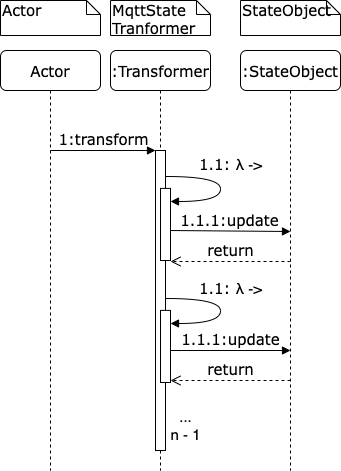
\includegraphics[width=14cm,height=8cm,keepaspectratio]{images/Transformation_old.png}
        \caption{Transformation über Switch-Case-Anweisung}
        \label{fig:sequenceTransformationOld}
    \end{figure}

\begin{lstlisting}[language=Java, frame=lines, xleftmargin=\parindent, style=algoBericht, label={code:switch-case}, captionpos=b, caption={Transformeation über eine Switch-Case-Anweisung}]
public class MqttTransformer extends AbstractTransformer<InnovationLabKA> {
    private final LogicHubState<InnovationLabKA> logicHubState;

    public void transform(String topic, String payload) {
        switch (topic) {
            case "InnovationLab/LogicHub/PersonOnDoor":
                logicHubState.setState((innovationLab) -> {
                    innovationLab.setPersonOnDoor(payload);
                    innovationLab.update();
                });
                break;
            case "InnovationLab/LogicHub/SR/GoTo":
                logicHubState.setState((innovationLab) -> {
                    innovationLab.setSRGoTo(payload);
                    innovationLab.update();
                });
                break;
        }    
    }
}
\end{lstlisting}
    Dieser Ansatz gibt eine Übersicht des Topics und der dafür vorgesehenen Zustandsänderung. Nachteile dabei sind jedoch, dass die Anweisungen 
    zunehmen, je mehr Regeln und dafür vorgesehen Zustandsänderungen hinzugefügt werden und die einmalige Verwendung der \acs{MQTT}-Topic-Zeichenkette. Dafür muss der 
    Anwender, um innerhalb einer Regel eine weitere Zustandsänderung vornehmen zu können, das Topic erneut aufgreifen und in Kenntnis des jeweiligen sein. Mit dem 
    Topic würde dann über den \acs{MQTT}-Producer eine Nachricht veröffentlicht werden, die die Aktion der Regeländerung steuert. 
    \\
    Diese umständliche Art und Weise galt es dem Anwender zu erleichtern, deshalb wurde ein zweiter Lösungsweg erarbeitet, der in folgendem Abschnitt 
    aufgezeigt wird.

    \subsubsection*{Transformationsobjekt mittels eigenem Objekt}
        In Opposition zu der Verwendung einer Switch-Case-Anweisung wird bei diesem Ansatz eine Klasse implementiert, mit der je nach Bedarf 
        weitere Objekte mit unterschiedlichen Werten erzeugt werden kann. Dabei werden in dem Konstrukt der Klasse die jeweiligen Parameter 
        definiert. Das zu erzeugende Objekt wird zur Laufzeit dem Framework übergeben und in einer Liste gespeichert, sodass das System damit arbeiten kann. 
        Die Parameter, die der Entwickler bestimmt, haben folgende Funktion:
        \begin{itemize}
            \item 1. Parameter: Hier wird das Topic übergeben. Der \acs{MQTT}-Subscriber prüft, ob das konsumierte Topic einem in der Liste definierten Topics entspricht.
            \item 2. Parameter: Hier wird der Key definiert. Das über das Topic mitgelieferte JSON-Konstrukt wird auf diesen key überprüft. Dessen Wert für den Zustandsraum relevant. Hierüber wird der Zustand des Objektes transportiert.
            \item 3. Parameter: Hier wird optional eine Liste übergeben, die nur bestimmte Werte für den Key zulässt, eine sogenannte \textit{White-List}.
            \item 4. Parameter: Hier wird der Name des Feldes im Zustandsraum wiedergegeben, sodass mittels Reflection der Wert im Zustandsraum adressiert werden kann.
            \item 5. Parameter: Hier wird der Name des Feldes der Komponente im Zustandsraum wiedergegeben, sodass mittels Reflection der Wert der Komponente im Zustandsraum adressiert werden kann.
        \end{itemize}
        Diese Werte bilden die Transformation, die ebenso für die inverse Transformation (siehe Abschnitt \ref{subsec:inverseTransformation}) gilt.
        Der Ablauf kann dem folgenden Sequenzdiagramm entnommen werden:
        \\
        \pagebreak
    \begin{figure}[hbt!]
        \centering
        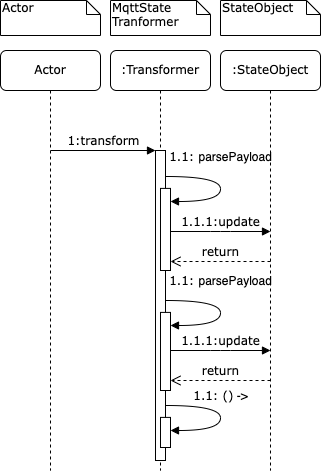
\includegraphics[width=14cm,height=9cm,keepaspectratio]{images/Transformation_new.drawio.png}
        \caption{Transformation über eigenes Objekt}
        \label{fig:sequenceTransformationNew}
    \end{figure}
    \\
    Um das Objekt zu erzeugen, muss der Entwickler lediglich das folgende Code-Beispiel verwenden und auf die entsprechenden Werte anpassen:
\begin{lstlisting}[language=Java, frame=lines, xleftmargin=\parindent, style=algoBericht, label={code:object}, captionpos=b, caption={Transformation über ein eigenes Objekt}]
public class InnovationLogicHubApplication {
    public InnovationLogicHubApplication() {
        ... 
        logicHub.addTransformation(
            new SimpleTopicTransformation(
                "InnovationLab/LogicHub/PersonOnDoor",
                "email",
                "personOnDoorEmail"
            )
        );
    }
}
\end{lstlisting}
    Für die jeweiligen Konfigurationsmöglichkeiten der Transformation gibt es drei Konstrukte, die jeweils benutzt werden können. 
    Neben der im Code-Beispiel (\ref{code:object}) aufgeführten Struktur gibt es die mit dem zusätzlichen Parameter der \textit{White-List} und 
    die dritte Möglichkeit, die zusätzlich den Namen eines Feldes innerhalb der Komponente wiedergibt. So können Objekte theoretisch in den Zustandsraum 
    aufgenommen werden, wovon allerdings zu aktuellem Zeitpunkt abgeraten wird. Die Begründung zu dieser Modellierung wird in dem Abschnitt 
    (\ref{subsec:modellierungsgrenzen}) aufgegriffen. 
    \\
    Der interne Ablauf des Frameworks unterscheidet sich bei beiden Transformationsmethoden in Nuancen, wie den beiden Sequenzdiagrammen 
    (\ref{fig:sequenceTransformationOld} und \ref{fig:sequenceTransformationNew}) zu entnehmen ist. Jedoch wird bei dem zweiten Ansatz 
    das Zustandsobjekt mittels Reflection manipuliert und anschließend als Änderung registriert und ausgeführt, während bei der ersten Methode 
    die Änderung direkt über die Lambda-Funktion gesteuert und ausgelöst wird. Dies hat für den Anwender keinerlei Auswirkung auf die 
    Funktionsweise des Frameworks, bei der Entscheidung war hingegen relevant, welcher Ansatz für den Entwickler den besseren darstellt. 
    An dieser Stelle bringt der zweite Ansatz Potentiale mit, die dem Entwickler die 
    Handhabung der Interaktionen formalisieren und erleichtern und zudem übersichtlicher gestalten.
    \\
    \linebreak
    Für die Vorteile, die der zweite Ansatz dem Entwickler gegenüber liefert, wurde dieser in dem Framework angewendet. 
    \\
    \linebreak
    Die Funktionsweise der Transformation ist demnach wie folgt umgesetzt:
    \\
    Die vorab definierten Transformationen des Entwicklers werden in einer Liste gespeichert, damit das darin enthaltene Topic mit dem vom \acs{MQTT}-Subscriber eingehenden 
    verglichen werden kann. Dafür wird über die Liste iteriert und jede Transformation, sowie deren zugewiesenes Topic geprüft. Sofern 
    es eine Übereinstimmung gibt, wird der Key-Wert ermittelt und als Nutzlast (\textit{Payload}) übergeben. An dieser Stelle wird der \textit{ReentrantLock} aktiviert 
    und die Feldmanipulation für den Wert durchgeführt, der mittels Nutzlast mitgegeben wurde. Nachdem die Zustandsänderung erfolgte, wird der \textit{Lock} deaktiviert und 
    die Zustandsänderung an die Logikschicht weitergegeben. Somit ist die Transformation für ein eingehendes \acs{MQTT}-Topic abgeschlossen. Der Ablauf kann dem Sequenzdiagramm (siehe Abbildung \ref{fig:kommunikationsequenz}) entnommen werden.  
    \\
    Die Funktion der inversen Transformation wird in folgendem Abschnitt erläutert.

\subsection{Inverse Transformation}
\label{subsec:inverseTransformation}
    Damit der Anwender des Frameworks bei der Regeldefinition einen geringen Aufwand erfährt und dennoch dadurch eine weitere 
    Zustandsänderung hervorrufen kann, findet an dieser Stelle eine inverse Transformation stattfinden. Dadurch wird anhand 
    der Zustandsänderung, die der Entwickler durch eine Funktion in der jeweiligen Regel vorgibt, die zugehörige Aktion mittels \acs{MQTT}-Nachricht 
    veröffentlicht. In Folge dessen muss der Entwickler bei der Implementierung einer Regel keine Kenntnis über das 
    \acs{MQTT}-Topic haben, lediglich muss das richtige Attribut im Zustandsraum angesprochen und geändert werden. 
    Ein konkretes Beispiel: 
    \\
    \linebreak
    Wird ein Lichtschalter eingeschaltet, so wird ein \acs{MQTT}-Topic konsumiert, dass den Zustandsraum ändert, indem 
    der Schalter betätigt wurde. Daraufhin wird eine Regel ausgeführt, deren Regelaktion die LED-Leuchte aktiviert. 
    Dementsprechend definiert der Entwickler eine Funktion, die den Wert des Lichtzustandes im Zustandsobjekt verändert. 
    Mit der Veränderung wird überprüft, um welches Attribut es sich im Zustandsraum handelt und wie sich der Wert geändert hat. 
    Wenn diese Überprüfung zutrifft, wird im Rahmen der inversen Transformation ein \textit{JSON}-Konstrukt generiert, welches 
    mit dem in der Transformation definierten Topic als \acs{MQTT}-Nutzlast an den \acs{MQTT}-Broker publiziert wird. Dabei handelt 
    es sich konkret um das Topic, auf das der \acs{MQTT}-Client der LED-Leuchte reagiert.
    Daraufhin wird die LED-Leuchte angeschaltet. 
    \\
    \linebreak
    Zusammengefasst wird mit der inversen Transformation vermieden, dass der Entwickler sich bei der Regelimplementierung neben der zu definierenden 
    Zustandsänderung zusätzlich um das veröffentlichen der jeweiligen Nachricht und das Verpacken in eine übertragbare 
    \textit{JSON}-Struktur kümmern muss. Des weiteren ist die Kenntnis über das Topics, unter dem die Nachricht 
    gesendet wird, ausschließlich in der Transformation von Nöten und muss nicht an mehreren Stellen konkret 
    aufgeschrieben werden. Dafür kann zu jeder Zeit die Liste der Transformationen genutzt werden, um das erforderliche Topic zu erhalten. 
    \\
    \linebreak
    Zu aktuellem Zeitpunk wird bei der inversen Transformation ein einfaches \textit{JSON}-Konstrukt erzeugt. Dafür wird der 
    \textit{Key}-Wert der Transformation und die Nachricht als Nutzlast verwendet. Zur Veröffentlichung der Nachricht unter einem 
    \acs{MQTT}-Topic, wird derzeit ausschließlich der \textit{Zigbee2MQTT}-Standard\footnote{Nutzung von Zigbee2MQTT. \url{https://www.zigbee2mqtt.io/guide/usage/mqtt_topics_and_messages.html} Besucht am 30.07.2022} 
    eingehalten. Dabei wird die Topic-Zeichenkette, die über das Transformationsobjekt abgerufen werden kann, um den Anhang (\textit{/set}) ergänzt. 
    Hierfür wird vorab das \textit{JSON}-Konstrukt generiert und mit den jeweiligen Werten belegt. Diese Struktur wird als Nutzlast mittels dem 
    Topic und dessen Anhang herausgegeben. Soll im Rahmen der Veröffentlichung einer Nachricht kein \textit{JSON}-Konstrukt sondern ein einzelner Wert 
    publiziert werden, so kann dies erfolgen, indem das Topic um den zugehörigen \textit{Key}-Wert der Transformation (\textit{/set/[Key-Wert]}) ergänzt wird. Ein Beispiel dazu:
    \\
    Eine LED-Leuchte wird mit einer Transformation mit den Werten \textit{"mqtt/topic/test"}, \textit{"key-state"} und dem Attribut \textit{"led-leuchte"} 
    definiert. Soll in dem Zuge die Nutzlast nur den Wert \textit{"on"} enthalten, so wird kein 
    \textit{JSON}-Konstrukt erzeugt sondern lediglich die Nachricht über das modifizierte Topic (\textit{"mqtt/topic/test/set/key-state"}) veröffentlicht. 
    \\
    \linebreak
    Resümierend gibt es im Kontext des \textit{Zigbee2MQTT} zwei Wege, um mit Geräten, die das ZigBee-Protokoll unterstützen, zu kommunizieren. Diese sind beide 
    über das Framework, somit auch über die inverse Transformation abgedeckt.

%
%Hierfür muss erneut eine  \acs{MQTT}-Nachricht 
%über ein bestimmtes Topic veröffentlicht werden. Diese Veröffentlichung findet im Rahmen der inversen Transformation statt Da diese Transformation bereits definiert wurde, ist innerhalb der Regel %ausschließlich die Zustandsänderung 
%zu definieren. Mithilfe der inversen Transformation wird anhand der Zustandsänderung die dementsprechende Aktion invertiert und unter 
%dem dafür vorgesehenen Topic eine Nachricht veröffentlicht, die die LED konsumiert und daraufhin das Licht angeschaltet. 

\subsection{Regeldefinition}
    Damit die Vorgaben für eine valide Regeldefinition eingehalten werden, wird dem Anwender mittels \textit{Template Methode}-Pattern 
    eine Schablone vorgegeben, die alle notwendigen Methoden vorgibt, die der Entwickler implementiert sollte. Zusätzlich gibt es eine Annotation, die 
    \textit{RuleAnnotation}, die eine Regel als solche kenntlich macht und die Implementierung der Methoden forciert. Die beiden wichtigsten Funktionen 
    innerhalb der Klasse, die durch die abstrakte Definition zum Softwareentwickler durchgereicht werden, ist zum einen die \textit{checkCondition}-Funktion und 
    zum anderen die \textit{ruleProcess}-Funktion. Innerhalb der erstgenannten Methode gibt der Anwender einen Sachverhalt vor, der zutreffen muss, sodass anschließend diese 
    Regel ausgeführt werden kann. Die Bedingung ist abhängig von dem Feld des Zustandsraumes und der Absicht für die der Regelprozess gestartet werden soll. Sofern die 
    Bedingung zutrifft, wird ein boolescher Werte (\textit{true}) zurückgeliefert, der die Regel ausführen lässt. Die ebenso wichtige Funktion des Regelprozesses beinhaltet die Schritte der 
    Regelausführung als klassische Methode, die keinen konkreten Wert zurückgibt, sondern lediglich die darin enthaltenen Punkte abarbeitet. An dieser Stelle können wiederum 
    weitere Zustandsänderungen implementiert werden. Dies ist abhängig von dem Inhalt der Regel und liegt ebenso in der Macht des Entwicklers. 
    \\
    Neben den beiden Hauptfunktionen, gibt es eine weitere Funktion, die den Auslöser der Regel definiert. Dieser dient dazu, um Regeln ggf. nur auslösen zu können, sofern ein bestimmter 
    Auslöser dafür aktiviert wurde. Zusätzlich gibt es weitere Funktionen, die reine Informationswerte halten, darunter den Regelnamen und die -beschreibung. Darüber hinaus hat der 
    Entwickler keinerlei Einschränkungen, das Regelobjekt ergänzend zu gestalten.

\subsection{Parallelisierung}
\label{subsec:parallelisierung}
    Bereits im Konzept wurde der Terminus der Parallelisierung und der Asynchronität aufgegriffen. Für das Auslösen einer Regel, wird der gesamte Prozess der 
    Bedingungsprüfung und der anschließenden Ausführung in einen \textit{Thread} ausgelagert, der durch einen 
    \textit{ThreadPoolExecutor}\footnote{Spezifikation des Thread-Pools. \url{https://docs.oracle.com/javase/7/docs/api/java/util/concurrent/ThreadPoolExecutor.html} Besucht am 27.07.2022} im java Code angestoßen wird. 
    Durch das Auslagern des konkreten Prozesses in einen eigenen \textit{Thread} können mehrere Regeln gleichzeitig ausgeführt werden, sofern die Bedingungsprüfung zutrifft und die 
    Regel ausgeführt wird. 
    In folge der Entscheidung, dass nach jeder Zustandsänderung immer alle Regeln durchlaufen werden, wäre eine sequenzielle Ausführung der Regeln sehr ineffektiv und langsam. Dadurch 
    würde sich das Durchführen von Regeln verzögern, bspw. wenn ein Licht eingeschaltet werden würde, davor allerdings noch zwei Regeln abgearbeitet werden müssten, die jeweils eine 
    Minute beanspruchen, würde sich das Licht erst nach zwei Minuten einschalten. Durch die Auslagerung des Regelmanagements in jeweils eigene \textit{Threads} entfällt die sequenzielle 
    Abarbeitung, da diese asynchron durchgeführt wird. Durch die Parallelisierung der Regelprozesse können gleichzeitig weitere Zustandsänderungen entstehen, die anschließend 
    wieder zusammengeführt werden und darauf gegebenenfalls weitere Regeln ausgeführt werden. An der Stelle der Zustandsänderung selbst greift der 
    Lock-Mechanismus, der durch einen \textit{ReentrantLock}\footnote{Spezifikation des Locks. \url{https://docs.oracle.com/javase/7/docs/api/java/util/concurrent/locks/ReentrantLock.html} Besucht am 27.07.2022} 
    realisiert ist. Dadurch wird sichergestellt, dass der Zustandsraum, der die aktuell geltenden Zustände wiedergibt, immer nur einen Änderungsvorgang durchführt. 

\subsection{Regelwerk -und management}
    Anknüpfend an die abgeschlossene Transformation wird nach der Zustandsänderung der Teil ausgeführt, der basierend auf der Zustandsänderungen 
    alle bekannten Regel überprüft und die zutreffenden ausführt. Grundlegend gilt hier, wenn eine Zustandsänderung keiner konkreten Regel zugeordnet 
    werden kann, fehlt entweder die dazugehörige Regel oder es liegt in der Absicht des Entwicklers, darauf keine Regel auszuführen. Wenn eine 
    Zustandsänderung mehrfach hintereinander erfolgt, wird diese, sofern keine weitere Bedingung darauf zutrifft, ohne Auswirkungen übertragen 
    und keine Regel ausgeführt. Damit jedoch voneinander unabhängige Regel parallel ausgeführt werden können, wird der Prozess der Regelüberprüfung und -durchführung 
    in einen \textit{Thread} ausgelagert, wie bereits im Abschnitt der Parallelisierung (siehe \ref{subsec:parallelisierung}) beschrieben. Der Ablauf kann dem 
    Sequenzdiagramm (siehe Abbildung \ref{fig:logiksequenz}) ab dem Schritt \textit{1.5:copyState} entnommen werden. 
    \\
    \linebreak
    Nach Implementierung der Funktionen des Frameworks ging es um die Umsetzung der Use Cases, um die Funktionalität des Systems zu testen 
    und Anhaltspunkte für die Evaluation (siehe Kapitel \ref{chap:evaluation}) zu schaffen. Der folgende Abschnitt behandelt die praktische 
    Umsetzung zweier Anwendungsfälle. 

\subsection{Implementierung von Anwendungsfällen}
    Zur Überprüfung des Frameworks wurden im Rahmen der Arbeit drei Anwendungsfälle implementiert, um anhand dessen die Funktionsweise 
    darzustellen. Zum einen wurde ein trivialer Fall, die Steuerung einer LED-Lampe über einen Schalter und ein Steckdosen-Funkmodul, umgesetzt, um einen Vergleich zwischen der 
    Regeldefinition in Home Assistant, \acs{OPENHAB} und der Steuerzentrale (InnovationLogicHub) ziehen zu können. Zum anderen wurden die beiden 
    Anwendungsfälle, die im Rahmen der Anforderungsanalyse (siehe Kapitel \ref{chap:anforderungsanalyse}) als Anwendungsfälle (\ref{sec:usecases}) definiert wurden, realisiert. 
    
    \subsubsection*{Lichtregelung}
    Der Lichtschalter-Anwendungsfall besteht darin, dass mittels einem physischen oder virtuellen Schalter eine LED-Leuchte eingeschaltet werden kann. Zur 
    Gegenüberstellung der Umsetzungen wurden jeweils die gleichen Komponenten im selben Netzwerk verwendet. Dadurch sind die identischen Voraussetzungen geschaffen. 
    Zu Beginn musste sichergestellt werden, dass die Komponenten mindestens das \textit{ZigBee}-Kommunikationsprotokoll unterstützen, damit über \textit{Zigbee2mqtt} 
    die Nutzung von \acs{MQTT} möglich war. 
    \\
    Im Rahmen dieser Arbeit wurden zu Anfang bereits Instanzen der beiden Plattformen, Home Assistant und \acs{OPENHAB}, gestartet, damit eine Grundlage zur Analyse und 
    Untersuchung der jeweiligen Plattformen gegeben ist. Diese wurden zur Umsetzung des einfachen Anwendungsfalls genutzt, um anschließend die 
    Resultate beurteilen zu können. Die Integration der Elemente in die jeweilige Plattform wird an dieser Stelle nicht weiter aufgegriffen, zur Veranschaulichung wird 
    lediglich die Regeldefinition aufgegriffen, damit diese kontrastiert werden können. Im Fokus steht jedoch die Umsetzung über die Steuerzentrale.
    \\
    \linebreak
    Unter Anwendung des Frameworks werden in folgendem Abschnitt die Schritte dargestellt, die notwendig sind, um den Anwendungsfall zu realisieren:
    \\
    Damit die Zustände der Komponenten abgebildet werden konnten, mussten diese im Zustandsraum hinterlegt werden. Unter der Berücksichtigung, dass der Schalter, sowie das Funkmodul 
    beide die trivialen Werte \textit{"on"} und \textit{"off"} über das Kommunikationsprotokoll versenden, wurden die Zustandsattribute jeweils als \textit{String}-Datentyp gewählt, um die 
    beiden Zustände abbilden zu können. Durch die Nutzung der \textit{lombok}-Bibliothek sind die \textit{Getter}- und \textit{Setter}-Methoden gegeben. 
    \\
    Anhand der definierten Zustandsattribute konnten anschließend die Transformationen für beide Komponenten implementiert werden. Dafür notwendig waren jeweils 
    die \acs{MQTT}-Topics, der Name des Wertes innerhalb des \textit{JSON}-Konstruktes, ggf. eine Liste der akzeptierten Zustandswerte und der Name des im Zustandsraum 
    definierten Feldes. Die Transformationen waren daraufhin dem Framework zu übergeben, damit diese in die dafür vorgesehene Liste aufgenommen und zur Laufzeit als Objekte 
    erzeugt werden konnten. Abschließend war die Regel zu definieren, darunter die zu prüfende Bedingung und die darauf folgende Aktion, das an- bzw. ausschalten des Lichtes über das 
    Steckdosen-Funkmodul. Die beiden Methoden sind überschaubar und mit weniger als fünf Zeilen Code implementiert. Dem Quellcode-Ausschnitt (siehe Anhang \ref{code:switch}) 
    sind die folgenden Methoden zu entnehmen.
    \\
    Die Umsetzung des Anwendungsfalls in Home Assistant stellte sich als umständlicher und aufwändiger dar. Hierbei war im Kontext des Home Assistant 
    eine übergreifende Automation, zwei Szenen (Aktionen) für das Schalten des Lichts und ein Auslöser für jede Aktion des Schalters zu definieren. Die Konfigurationsdatei 
    erstreckt sich über 50 Zeilen, in denen die eigentliche Funktion definiert wird. Das Erstellen der Automatisierung über die Nutzeroberfläche gestaltet sich einfacher, dennoch 
    aufwändig mit vielen Interaktionen. Ergänzend dazu ist dem Anhang ein Ausschnitt der Konfigurationsdatei beigefügt (siehe Anhang \ref{code:hoasAutomation}).
    \\
    \linebreak
    Ähnlicher Konfigurationsaufwand war bei der Umsetzung in \acs{OPENHAB} über die Benutzeroberfläche festzustellen. Das skriptbasierte Definieren von Regeln erfordert eine 
    hohe Lernkurve, da die Semantik  des \textit{ECMAScript} oder die Funktionsweise von bspw. \textit{Blockly} erst erlernt und verstanden werden muss. Die Regeldefinition 
    mittels der \textit{Rule \acs{DSL}} hingegen kann mit der der Steuerzentrale verglichen werden. Diese ist in ähnlich wenigen Schritten realisiert. Der 
    Quellcode-Ausschnitt zeigt den Umfang der Regel über die \acs{OPENHAB} \acs{DSL} (siehe Anhang \ref{code:openhabSwitch}). 
    \\
    \linebreak
    Die Umsetzung der folgenden Anwendungsfälle erfolgte ausschließlich über die Steuerzentrale.

    \subsubsection*{Check-in mit einem Service-Roboter}
        Die Handlungsschritte, um einen Anwendungsfall mit dem Framework zu realisieren, sind grundlegend immer die gleichen. Je nach Bedarf sind mehrere 
        Aktionen notwendig. Damit alle, für den Fall, notwendigen Zustände abgedeckt sind, wurden diese in dem Zustandsraum hinterlegt. Zu den notwendigen Attributen 
        zählen unter anderem die E-Mail-Adresse, bzw. der Name der authentifizierten Person, die Verfügbarkeit des Service-Roboters, sowie dessen 
        verfügbaren Prozesse. Anschließend wurden die Transformationen definiert. 
        \\
        \linebreak
        Sobald eine Person über die Kamera authentifiziert wurde, wird ein \acs{MQTT}-Topic gesendet, welches als Nutzlast ein \textit{JSON}-Konstrukt mit einem Zeitstempel, den 
        Vor- und Nachnamen, sowie die E-Mail-Adresse der Person übergibt. Anhand dessen wird im Zustandsraum der Wert der E-Mail geändert, worauf die Regeln auf ihre 
        Bedingung überprüft werden. Dabei wird die Regel zum Begrüßen und einchecken des Gastest gestartet. Hierfür wird der Service-Roboter an die Tür geschickt, an der er den 
        Gast empfängt. Während der Roboter an die Tür fährt, checkt er die Buchungen und überprüft, ob die Person einen Platz gebucht hat. Dort angekommen, wird die Person zuerst 
        begrüßt. Nachdem der Gast empfangen und eine Buchung gefunden wurde, fragt der Service-Roboter, ob er den Gast einchecken soll. Dieser kann die Frage beantworten. 
        Wird die gestellte Frage bejaht, so checkt der Service-Roboter die Person in dem Büroplatzbuchungssystem ein.  
        \\ 
        Falls bei der Abfrage des Service-Roboters keine Buchung gefunden wurde, wird der Gast aktuell darum gebeten, nachträglich einen Platz zu buchen und darauf einzuchecken. 
        Die Regelabfolge kann zusätzlich dem Sequenzdiagramm (siehe Abbildung \ref{fig:sequenceRuleGreet}) entnommen werden.
        \begin{figure}[hbt!]
            \centering
            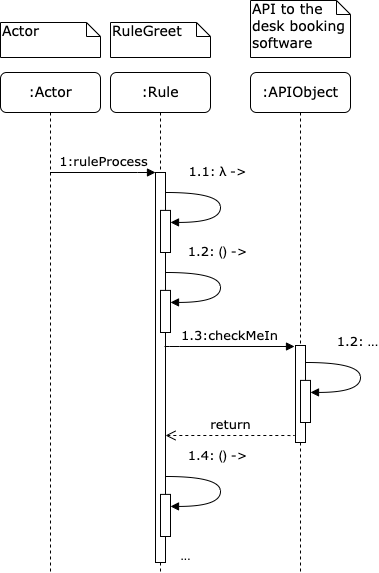
\includegraphics[width=14cm,height=12cm,keepaspectratio]{images/sequence_rule_temi_greet.png}
            \caption{Check-in Regelablauf (RuleProcess)}
            \label{fig:sequenceRuleGreet}
        \end{figure}
        \\
        %\pagebreak
        %\linebreak
        Der Check-in wurde im Rahmen dieser Arbeit als eine Handlungskette implementiert, da der Roboter zu aktuellem Zeitpunkt noch keine interaktiven Statusmeldungen geben kann. Dies 
        Bedeutet, dass derzeit Befehle entgegengenommen werden können, darauf allerdings keine Rückmeldung erfolgt. Somit ist ein Zustandsaustausch in Echtzeit nicht möglich. 
        Aus diesem Grund wurde nach jedem ausgehenden Befehl ein Intervall eingebaut, damit die Regel sequenziell abgearbeitet werden kann. Dafür wurden Zeitspannen definiert, die 
        der Roboter in etwa braucht, um einen Ortswechsel, bzw. einen Sprachbefehl durchzuführen. Eine alternative Lösung, sofern der Service-Roboter Statusmeldungen geben 
        kann, wäre die feingranularere Aufteilung von einzelnen Prozessen, sodass erst nach erfolgreicher Rückmeldung des Roboters der weitere Schritt eingeleitet werden würde.
        \\
        \linebreak
        Wird bspw. ein Sprachbefehl ausgeführt, so wird innerhalb der Regel über eine \textit{Lambda}-Funktion der Zustandsraum erneut geändert, wodurch die inverse Transformation 
        die Zustandsänderung überprüft und anhand dessen den Sprachbefehl über ein \acs{MQTT}-Topic an den Broker sendet. Hierbei reagiert der Roboter auf das Topic und führt 
        den Sprachbefehl aus. Diese Aktion ist dem Sequenzdiagramm (\ref{fig:sequenceRuleGreet}) unter anderem in den Schritten \textit{1.2:() ->} zu entnehmen. 
        \\
        Der Anwendungsfall wurde erfolgreich umgesetzt und konnte mit dem realen Service-Roboter getestet werden. Für die 
        Usability-Tests \ref{sec:usabilitytest}, zur Überprüfung der Nutzbarkeit, wurde ein \textit{Mock}\footnote{Simulierte Objekte in der Objekt-orientierten Programmierung. \url{https://en.wikipedia.org/wiki/Mock_object} Besucht am 02.08.2022} 
        des Service-Roboters entwickelt, um die Interaktionen simulieren zu können.
    
    \subsubsection*{Notfall-Evakuierung mit einem Service-Roboter}
        Der Anwendungsfall der Notfall-Evakuierung enthält ähnliche Handlungsschritte als die des Check-ins, weswegen dieser nicht in die 
        Tiefe aufgegriffen wird. Die Prozessschritte sind ebenso möglich umzusetzen und wurden auch im Rahmen dieser 
        Arbeit umgesetzt. Der Ablauf gestaltet sich ähnlich zu dem im Sequenzdiagramm \ref{fig:sequenceRuleGreet} dargestellt. 
        Der Roboter selbst ist aktuell nicht in der Lage Personen zu erkennen. Um dies zu vereinfachen, wurde im Rahmen dieser Arbeit 
        lediglich ein gebuchter Platz angefahren und die Warnmeldung ausgeführt. Dies erfolgt für jeden gebuchten Platz des Erdgeschosses 
        im Büro.
        
    \section{Fazit der prototypischen Implementierung}
        % Entscheidung für die Nutzung von Reflection. Begründung: Überprüfung der Werte im Zustandsraum, welche sich geändert haben. 
        %Und zur Nutzung der inversen Transformation, um an einer Stelle die Topics etc. zu definieren.
        Die Anwendungsfälle konnten wie erwartet umgesetzt werden und zeigen, dass die konzeptionellen Entscheidungen eine Grundlage für das 
        Framework darstellen. Die Regeln selbst können je nach Anwendungsfall beliebig definiert werden. An dieser Stelle werden dem 
        Entwickler alle Möglichkeiten offengelassen, dadurch erfährt dieser keine Einschränkungen. Des weiteren ist der Schnitt zwischen 
        Anwender und Framework klar gegeben, indem der Softwareentwickler sich ausschließlich um die Regeln, Transformationen und Zustandsattribute 
        kümmern muss. Entscheiden ist die Gegebenheit eines \acs{MQTT}-Brokers, da ohne diesen das Framework keine Verbindung aufbauen und so nicht an 
        einem Datentransfer teilnehmen kann. 
        \\
        \linebreak
        Mit der Konzeption der Transformation wird bereits zu Anfang ein zentraler Punkt gegeben, mit dem der Anwender alle notwendig Informationen 
        bündeln und dem Frameworks zur Verfügung stellen kann. Anhand dieses Beschlusses kann der Entwickler die Zuordnung treffen, bspw. durch welches 
        eingehende \acs{MQTT}-Topic welches Attribut im Zustandsraum geändert werden soll. Mit der Entscheidung zur Nutzung der generischen Programmierung 
        und somit der flexiblen Gestaltung des Zustandsraumes, musste überlegt werden, wie dieses Objekt dennoch überwacht und manipuliert werden konnte. 
        Hierfür wurde die Java Reflection genutzt, die eine sehr mächtige Funktion der Java-Programmierung darstellt, dennoch für die Nutzung aktuell 
        Grenzen einräumt, die im Rahmen der Konzeption hingenommen wurden, allerdings keine Einschränkung bewirken. Trotz dessen kann durch die Einhaltung 
        von den Modellierungsvorgaben (\ref{subsec:modellierungsgrenzen}) die Grenze umgangen werden und so die Anwendungsfälle, die im Rahmen der Arbeit 
        definiert wurden, bzw. in der Umgebung eines smarten Büros auftreten können, umgesetzt werden. Entscheidend ist dabei die Definition der 
        Transformation, sowie die der Regel selbst. 
        \\
        \linebreak
        Der Prototyp erfüllt alle Voraussetzungen, um die definierten Anwendungsfälle umzusetzen.
    
    \subsection{Modellierungsvorgaben und -grenzen}
    \label{subsec:modellierungsgrenzen}
        Aus Sicht des Anwenders hat dieser drei Stellen, die in seiner Verantwortung liegen. Damit steht  
        dem Entwickler alles zur Verfügung, was er benötigt, um seine Anwendungsfälle nach den Bedürfnissen zu implementieren. 
        \\
        \linebreak
        In der Klasse, in der die Zustandsattribute abgebildet werden, ist das Nutzen von einfachen Attributen vorgesehen. Es können 
        zwar Objekte hinzugefügt werden, dies erschwert jedoch die Überprüfung, ob Änderungen darin vorgenommen wurden. 
        Dies ist zum Teil der Reflection geschuldet, da im Zustandsraum lediglich die Referenz des zur Laufzeit erzeugten Objektes 
        steht und zum anderen, da bei der Kopie des Zustandsobjektes eine neue Objektreferenz geschaffen wird, die als Änderung 
        registriert wird. Das bedeutet jedoch nicht, dass immer eine Änderung des Objekts hervorgerufen wurde. Ebenso müsste sichergestellt 
        werden können, um welches Objekt es sich handelt. Um dies sicherzustellen, wäre ausschließlich das Hinzufügen von Komponenten im 
        Zustandsraum zugelassen. Damit dies jedoch umgangen werden kann, wird vorerst die Nutzung von einfachen Attributen, darunter 
        \textit{String}, \textit{Integer}, \textit{Double}, \textit{boolean} und \textit{Long} empfohlen. Andere Felder können zwar hinzugefügt werden, 
        diese werden jedoch nicht vom Framework berücksichtigt.
        \\
        \linebreak
        Die Transformation gibt ein klar definiertes Konstrukt. Dafür gibt es Zwei Klassen, die implementiert werden können, die 
        jeweils die Oberklasse \textit{AbstractTopicTransformation} erweitern. Zum einen die Transformation ohne 
        optionale \textit{White-List} von zugelassenen Werten und zum anderen die, in der eine solche Liste übergeben werden kann. Über die 
        \textit{addTransformation}-Funktion wird zur Laufzeit das Transformationsobjekt erzeugt. Die Inhalte sind klar vorgegeben (siehe Abschnitt \ref{subsec:transformation}) 
        und müssen vom Entwickler entsprechend definiert und erzeugt werden.
        \\
        \linebreak
        Die Definition einer Regel sieht vor, dass die Bedingung, die zutreffen muss, auf eine Zustandsänderung zutreffen muss. Der Regelprozess kann vom Anwender 
        frei implementiert werden. Zum Erstellen einer Regel ist zu Anfang sicherzustellen, dass diese von der Abstrakten Regel klasse erbt. So kann die Regel einer 
        Oberklasse zugeordnet werden und vom Framework als solche erkannt werden. Zusätzlich dazu, gibt es für die wichtigen Funktionen, die eine Regel zum 
        Implementieren bereitstellt, eine Annotation. Diese geben syntaktische Metadaten vor, die die richtige Implementieren der Funktionen forciert. Die 
        Annotation muss beim erstellen einer Klasse über der Funktion hinzugefügt werden. Dem Quellcode-Ausschnitt im Anhang (siehe \ref{code:switch}) ist diese 
        syntaktische Hilfestellung zu entnehmen. Wichtig ist ebenso, dass nach der Definition einer Regel diese auch dem Framework mittels der \textit{addRule}-Funktion 
        übergeben wird. 
        \\
        Diese Anmerkungen sind bei der Nutzung des Frameworks zu berücksichtigen, damit das Framework entsprechend arbeitet und die Regel und Prozesse ausführt. 
    %WICHTIG: ZUSTANDSRAUM MODELLIERUNG VON KOMPONENTEN, BZW. OBJEKTE SIND MÖGLICH, 
    %Problematisch dabei ist die Prüfung der Zustandsänderung, da bei jeder Kopie eine neue 
    %Referenz der Komponente erzeugt wird, die eine Zustandsänderung unter dem Feld simuliert (vorgibt) ohne das diese tatsächlich stattgefunden hat.
    %UND DA DIE INVERSE TRANSFORMATION ZUM AUSLÖSEN VON AKTIONEN NUR DIE OBERSTE EBENE DES ZUSTANDSRAUMES ANSCHAUT UND ÜBERPRÜFT.
    % An dieser Stelle müsste feingranularer überprüft werden, dass allerdings nicht funktioniert. Heißt: aktuell werden nur die 
    %Änderungen auf der obersten Ebene überprüft das Absteigen in Objecte ist dabei nicht möglich, da das Object im Framework erst zur Laufzeit bekannt ist.
    
    % IST ABER AUCH NICHT NÖTIG, DA ALLE 
    %NOTWENDIGEN GEGENSTÄNDE ÜBER EINEN ODER MEHRERE ATTRIBUTE IM ZUSTANDSRAUM ABGEBILDET WERDEN KÖNNEN. BSP.? 
    % UND DIE ATTRIBUTE, BZW. DIE FELDER ÜBER DIE TRANSFORMATION GEBUNDEN WERDEN. 
    
    %Grenzen 
    %Modellierungsempfehlungen - Regel, Bedingung und Zustandraum 
    %Worauf man achten soll, wenn man ein neues Szenario abbildet. 
    %Modellierungsmöglichkeiten des Frameworks.
